\section{Procedure}
\label{sec:procedure}

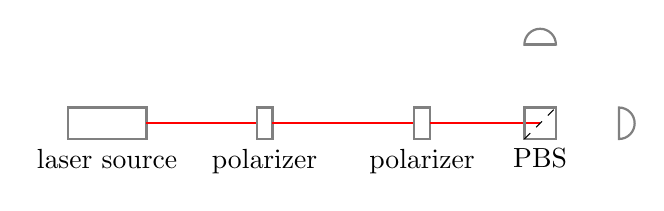
\begin{tikzpicture}
  \draw[gray, thick] (-3.5,-0.2) rectangle (-2.5,0.2); 
  \node[below] at (-3,-0.2) {laser source};
  \draw[red, thick] (-2.5,0) -- (-1.1,0); 

  \draw[gray, thick] (-1.1,-0.2) rectangle (-0.9,0.2); 
  \node[below] at (-1,-0.2) {polarizer};
  
  \draw[red, thick] (-0.9,0) -- (0.9,0); 

  \draw[gray, thick] (0.9,-0.2) rectangle (1.1,0.2); 
  \node[below] at (1,-0.2) {polarizer};

  \draw[red, thick] (1.1,0) -- (2.5,0); 
  \draw[gray, thick] (2.3,-0.2) rectangle (2.7,0.2); 
  \draw[dashed] (2.3,-0.2) -- (2.7,0.2);
  \node[below] at (2.5,-0.2) {PBS};

  \draw[gray, thick] (2.3, 1) -- (2.7,1);
  \draw[gray, thick] (2.3,1) -- (2.7,1) arc(0:180:0.2) --cycle;

  \draw[gray, thick] (3.5,0.2) -- (3.5,-0.2) arc(-90:90:0.2) --cycle;
\end{tikzpicture}

